%!TEX root = /Users/velrok/Dropbox/TheoInf Seminar/Ausarbeitung/Main.tex
\section{Ähnlichkeitstheorie} % (fold)
\label{sub:Aehnlichkeitstheorie}

Die Ähnlichkeitstheorie besagt, das sich die Eigenschaften einer Modal-Logik in der Relation der entsprechenden Kripkestrucktur widerspiegeln und vis versa. 
Dies schafft einen neuen Zugang zum Design von Modal-Logiken. 
In manchen Fällen mag es einfacher sein in den notwendigen Eigenschaften in Form von Formel-Schemata zu denken, in anderen ist es evtl. einfacher das Problem über die Relation zu verstehen. 
Im Folgenden wird gezeigt, wie die einzelnen Eigenschaften mit der Kripke-Struktur-Relation zusammen hängen.


\paragraph{Zusammenhang zwischen der Relation $R$ und den validen \formelSchemata}

Wir haben in \Abs{festlegung_von_attibuten_mit_R} den Zusammenhang zwischen der Transitivität von $R$ und der Validität der Formel \vierFormel durch die Intuition begründet, dass die \emph{positive Introspektion} gilt.
Es wird nun gezeigt, dass sich dieser Zusammenhang mathematisch beweisen lässt.
Dazu muss zunächst der Begriff \emph{Frame} eingeführt werden:

\begin{definition}
	\label{def:frame}
	Ein Frame $\Fancy{F} = (W,R)$ ist eine Menge von Welten $W$ und eine binäre Relation $R$ auf $W$.
	\cite[S.322]{huth2004logic}
\end{definition}

\emph{Frames} kann man sich also als \KS ohne \emph{Labeling-Funktion} vorstellen.
Damit beschreiben sie die selbe Struktur, jedoch unabhängig von der Konkreten Wissensbasis, sprich den geltenden Facken in jeder Welt.
Damit übernehmen sie in Kripke-Strukturen die selbe Rolle wie \formelSchemata in \MLFn .

\begin{definition}
	\label{def:frame_erfuellt}
	Ein Frame $\Fancy{F}$ erfüllt eine modal logische Formal $\psi$, wenn für jede \fachwort{Labelfunktion} $L: W \rightarrow \Fancy{P}(Atome)$ und jedes $w \in W$, es der Fall ist, dass $\Fancy{M},w \vDash \psi$ gilt. $\Fancy{M}$ ist das Model: $\Fancy{M} = (W,R,L)$.
	In diesem Falle schreiben wir $\Fancy{F} \vDash \psi$.
	\cite[S.322f]{huth2004logic}
\end{definition}

Wenn ein Frame eine Formel erfüllt erfüllt es auch das entsprechende Schema.

\begin{figure}[h!]
	\label{fig:Kripke02}
	\centering
	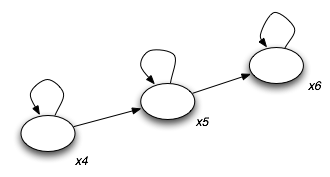
\includegraphics[width=10cm]{Images/Kripke02}
	\caption{Beispielframe}
\end{figure}

\begin{figure}[h!]
	\label{fig:Kripke03}
	\centering
	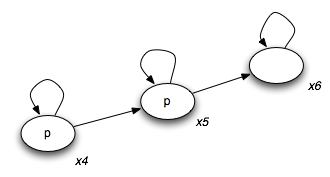
\includegraphics[width=10cm]{Images/Kripke03}
	\caption{Gegenbeispiel}
\end{figure}


Beispiel dafür (5.12)
\begin{itemize}
	\item erfüllt die \TFormel
	\item Bew: jede welt mit beligbiger L erfüllt das
	\item z.z.: wenn $x \VDash \Box p$ dann $x \VDash p$
	\item erfüllt nicht \vierFormel (Gegenbeispiel)
\end{itemize}


Theorem warum das Bsp. Frame \TFormel erfüllt aber \vierFormel nicht:

Beweis dafür:

Behauptung das Tabelle s.u. gilt

\todo{Tabelle über name schema und R Eigenschaften}











\begin{itemize}
	\item Was genau ist das? : Ein bewiesenes Theorem.
	\item Wie ist das begründet? : Ursprung Intuition, kann aber bewiesen werden.
	\item Wie werden die Definitionen genutzt? : Frames sind eine veralgemeinerung von Modellen. Können analog zu formel Schemata in Formeln gesehen werden.
	\item Welche Behauptungen werden aufgestellt? : siehe tabelle 5.12
	\item Wie werden diese Bewiesen? : Ringschluss S. 325
	\item Was sind Frames? : die analogie zu Formel Schemeta. \KS ohne Labels
	\item Wozu brauch man Frames? : für die Beweise der Theoreme. Um zu zeigen, dass ein Model eine Eigenschaft hat die unabhängig ist von der Konkreten Wissensbasis -> alg. gültig.
\end{itemize}











\todo{mehr schreiben}

% subsection Aehnlichkeitstheorie (end)
